\documentclass[reportComp]{thesis}
\usepackage[table,pseudo]{mypackage}

\title{模式识别作业Chap 7}
\school{数据科学与计算机学院}
\author{陈鸿峥}
\classname{17大数据与人工智能}
\stunum{17341015}
\headercontext{模式识别作业}

\begin{document}

\maketitle

\begin{question}[\textsection 7 Q3]
图7-2左边的能量地形曲面过分复杂,因下述原因容易误导读者:
\begin{figure}[H]
\centering
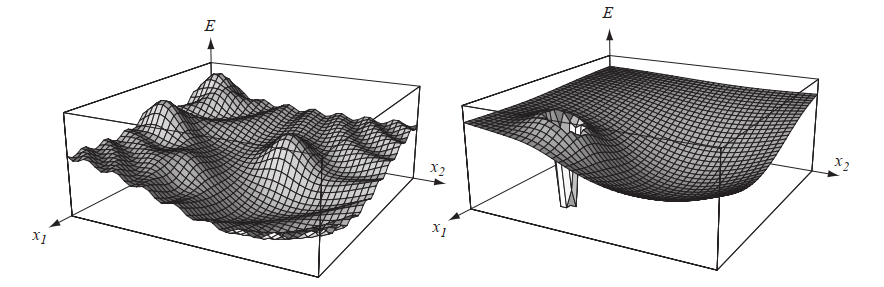
\includegraphics[width=0.8\linewidth]{fig/fig7-2.png}
\end{figure}
\begin{itemize}
	\item [(a)] 对式(1)的优化问题,讨论图中的连续空间与离散空间的差异。
	\item [(b)] 图中示出在空间的中部有一个局部能量极小点,问对于离散空间,是否存在中部的极小点?
	\item [(c)] 如果令坐标轴是连续的状态变量$s_i$(比如在均场退火中),若$s_i$服从sigmoid函数(图7-5),试问能量地形是否可以是非单调的,就像图7-2那样?
\end{itemize}
\end{question}
\begin{answer}
\begin{itemize}
	\item [(a)] 在(1)式的连续空间下,变量只能取值$\pm 1$,进而能量函数也是空间中孤立的点,不会出现图中所示的连续曲面。
	\item [(b)] 不可能,如果变量只能取值$\pm 1$的话,所有可行解都只会落在$\pm 1$圈定的超立方体的顶点上,而不会在内部。
	\item [(c)] 不一定。如果沿着平行于坐标轴方向将能量函数映射到3维空间,则能量地形一定是单调的,因为sigmoid函数是单调的,而此时只有一个变量在变化;若不沿着坐标轴方向做投影,则能量地形不一定是单调的,因为涉及到多个sigmoid函数的叠加。
\end{itemize}
\end{answer}

\begin{question}[\textsection 7 Q10]
考虑一个2-输入,1-隐单元,1-输出的全互连Boltzmann网络,试着手工构造所有权值,使之实现XOR。
\end{question}
\begin{answer}
不妨设符合下面情况的Boltzmann网络能量最小(即4个训练样本),其中$s_3$的值为人为给定
\begin{center}
\begin{tabular}{cc|c|c}\hline
输入$s_1$(可见) & 输入$s_2$(可见) & 隐层$s_3$(非可见) & 输出$s_4$(可见)\\\hline
 $+1$ & $+1$ & $+1$ & $-1$\\
 $+1$ & $-1$ & $-1$ & $+1$\\
 $-1$ & $+1$ & $-1$ & $+1$\\
 $-1$ & $-1$ & $-1$ & $-1$\\\hline
\end{tabular}
\end{center}
并考虑以下权值及偏置
\[\begin{array}{llllllll}
w_{13} &= 1 & w_{23} &=1 &\theta_{3} &= -1 & \theta_{4} &=-1/2\\
w_{14} &= 1/2 & w_{24} &=1/2 & w_{34} &=-1
\end{array}\]
\begin{figure}[H]
\centering
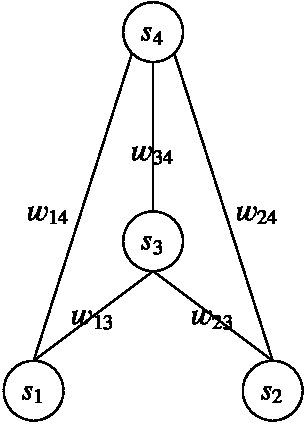
\includegraphics[width=0.25\linewidth]{fig/Q10.pdf}
\end{figure}

进而根据Boltzmann网络能量的表达式
\[E=-\left(\sum _{{i<j}}w_{{ij}}\,s_{i}\,s_{j}+\sum _{i}\theta _{i}\,s_{i}\right)\]
可求得
\begin{center}
\begin{longtable}{cccc|c}\hline
$s_1$ & $s_2$ & $s_3$ & $s_4$ & $E$\\\hline
$1$ & $1$ & $1$ & $1$ & $-0.5$ \\
$1$ & $1$ & $1$ & $-1$ & $-1.5$ \\
$1$ & $1$ & $-1$ & $1$ & $-0.5$ \\
$1$ & $1$ & $-1$ & $-1$ & $2.5$ \\
$1$ & $-1$ & $1$ & $1$ & $2.5$ \\
$1$ & $-1$ & $1$ & $-1$ & $-0.5$ \\
$1$ & $-1$ & $-1$ & $1$ & $-1.5$ \\
$1$ & $-1$ & $-1$ & $-1$ & $-0.5$ \\
$-1$ & $1$ & $1$ & $1$ & $2.5$ \\
$-1$ & $1$ & $1$ & $-1$ & $-0.5$ \\
$-1$ & $1$ & $-1$ & $1$ & $-1.5$ \\
$-1$ & $1$ & $-1$ & $-1$ & $-0.5$ \\
$-1$ & $-1$ & $1$ & $1$ & $5.5$ \\
$-1$ & $-1$ & $1$ & $-1$ & $0.5$ \\
$-1$ & $-1$ & $-1$ & $1$ & $-2.5$ \\
$-1$ & $-1$ & $-1$ & $-1$ & $-3.5$ \\\hline
\end{longtable}
\end{center}
满足(隐层状态不同可取等,但输出状态为严格不等式)
\[\begin{aligned}
E_{\{+1,+1,+1,-1\}} &\leq E_{\{+1,+1,\cdot,\cdot\}}\\
E_{\{+1,-1,-1,+1\}} &\leq E_{\{+1,-1,\cdot,\cdot\}}\\
E_{\{-1,+1,-1,+1\}} &\leq E_{\{-1,+1,\cdot,\cdot\}}\\
E_{\{-1,-1,-1,-1\}} &\leq E_{\{-1,+1,\cdot,\cdot\}}
\end{aligned}\]
即每个样本输入输出在对应的4种能量构型中都最小,进而该网络可以用于计算XOR函数。
\end{answer}

\end{document}